\documentclass[withoutpreface,bwprint]{cumcmthesis} 
%去掉封面与编号页

\usepackage[framemethod=TikZ]{mdframed}
\usepackage{url}   % 网页链接
\usepackage{subcaption} % 子标题
\usepackage{float}
\title{中小微企业的信贷决策问题}

\tihao{C}
\baominghao{4321}
\schoolname{山东大学大学}
\membera{桂孝强 主建模}
\memberb{潘鹏飞 主编程}
\memberc{郑子新 主论文}
\supervisor{ }
\yearinput{2020}
\monthinput{09}
\dayinput{10}

\begin{document}
 \maketitle
 \begin{abstract}
    中小微企业在我国逐渐成为推动国家经济繁荣的中坚力量,但与其资金短缺、融资困难的发展现状的矛盾却愈加突出。本文针对银行对
    中小微企业信贷策略问题,基于层次分析法、正态分布、非线性规划,建立了数学模型,给出了银行在固定
    年度贷款额度下是否放贷及贷款额度、利率、期限等信贷策略的方案以及面对突发情况下的调整策略。
    
    针对问题一,本文分析了影响企业信贷风险的七大因素,归结为实力模型、供求关系模型以及信誉评级三大指标,再基于层次分析法
    得到信贷风险评估模型,根据信贷风险指标来直接判断银行能否为该企业放贷。
    根据不同的行业受不同行业系数的影响,建立安全额度模型,表示在该额度及以下能够确保风险在可控范围内,结合信贷风险阈值
    求出该企业的贷款额度区间,即安全贷款额度至最大贷款额度;在基准利率的基础上,综合信誉评价与信贷风险指标
    对信誉好、信贷风险小的企业给予利率优惠。最终建立了以贷款额度、信贷风险指标、客户流失率在不同决策下形成的最大
    利润为目标函数的非线性规划模型。 

    针对问题二,以问题一中已经建立的指标较为完善的信贷策略模型为基础,在此模型上依据具体情况进行应用求解。由于
    给定数据的企业不包含信贷记录,因此我们依据众数原则将企业的信誉评级均确定为B级。考虑到所有企业最大贷款额度之和可能少于
    银行年度贷款固定总额,我们可以采用正态分析法对其进行调整,以平均贷款额度为期望值,使得企业贷款额度与银行年度贷款固定总额相关联。
    整理相关数据,应用银行决策模型,即可给出银行在年度信贷总额为1亿元时对这些企业的信贷策略。

    针对问题三,我们以新冠肺炎疫情为具体实例代表突发状况对各企业的影响,收集统计不同行业的收入变化率,根据变化率,利用层次分析法
    对问题一所建立的模型进行修改调整。收入变化率为正的企业表示它们适应了突发状况并产生了正面影响,而变化率为负的企业则代表着受到了
    突发状况的负面影响,应对这些企业给予一定的扶持利率优惠。同时由于收入的变化需要重新对各企业的信贷风险
    进行评估,进而获得新的贷款额度范围。这样的方案既能帮助收入变化率为负的企业,发挥其对于民生和实体经济稳定发展的支持作用,也能根据
    实际情况对模型中的因素进行适当调整,获得尽量大的盈利。另外,我们还定性地对不同的企业类别承受突发状况的风险能力进行了分析,更加全面地
    得到针对突发情况的调整改进模型。

    \keywords{层次分析法\quad   安全额度\quad  正态分布\quad 非线性规划 \quad 信贷扶持}
    \newpage
\end{abstract}

\section{问题重述}
\subsection{问题背景}
近年来,我国营商环境不断改善,中小微企业的总量规模不断地扩大,在国民经济和社会发展中的作用日益显著,成为国民经济的重要支柱。
图\ref{fig:propotion}是2018年末大中小微企业占全部规模企业法人单位比额示意图。

\begin{figure}[H]
    \centering
    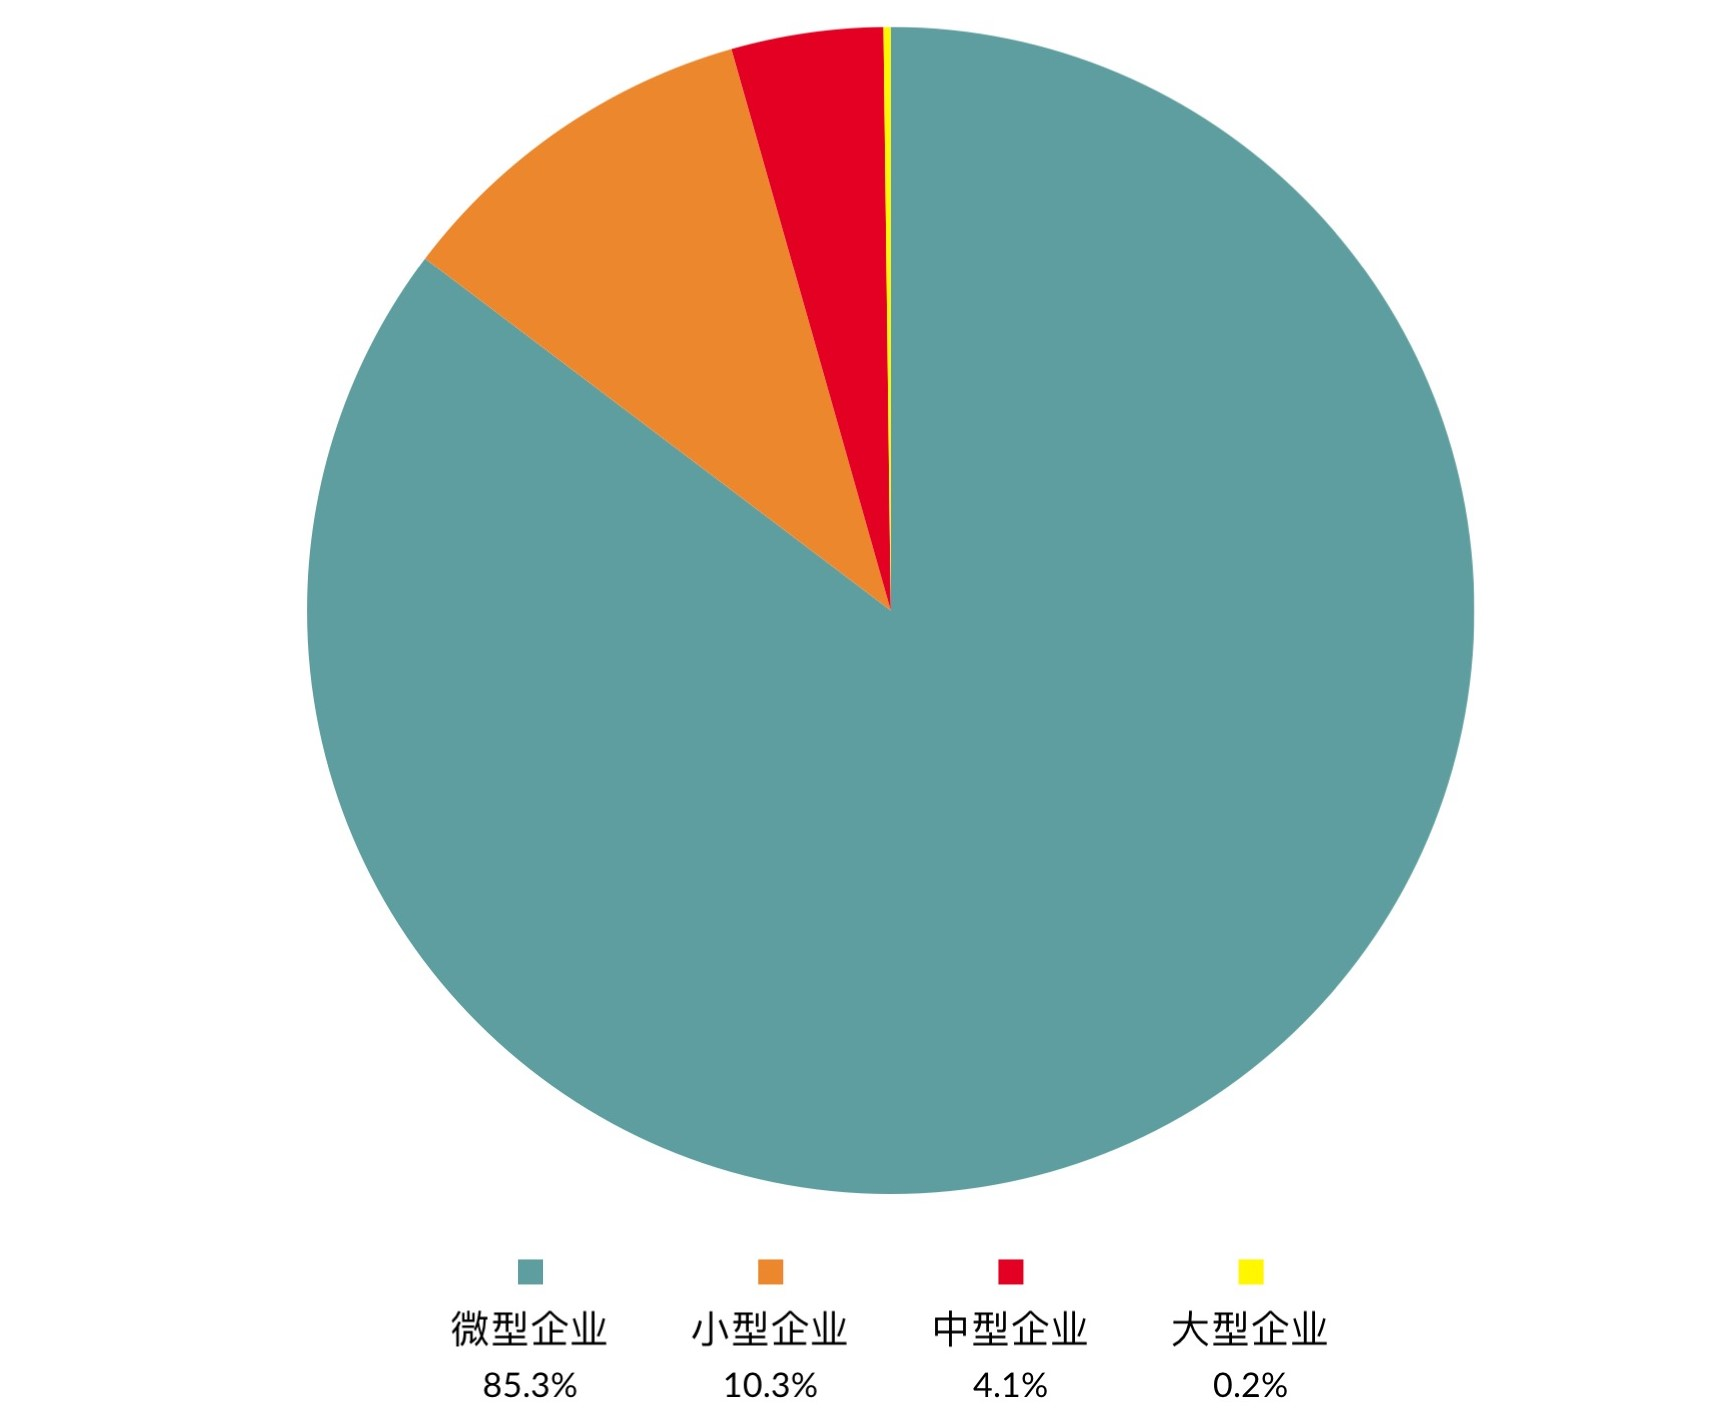
\includegraphics[width=.6\textwidth]{propotion .jpg}
    \caption{2018年末大中小微企业占全部规模企业法人单位比额}
    \label{fig:propotion}
\end{figure}

其中,中小微企业占全部规模企业法人单位比额达到的99.8\%,在扩大就业、推动经济增长等方面具有不可替代的作用,因此,支持
中小微企业的发展具有全局和战略性的重要意义。而在实际中,资金短缺仍然是中小企业发展面临着的瓶颈之一。由于抵押资产要求、企业规模
限制等门槛,银行通常根据信贷政策、企业的交易票据信息和上下游企业的影响力,向实力强、供求关系稳定的企业提供贷款,并可以对信誉高、
信贷风险小的企业给予利率优惠。

\subsection{问题提出}
根据以上背景并结合实际,以及给出的三个附件,建立数学模型研究下列问题:

(1) 对附件1中123家企业的信贷风险进行量化分析,给出该银行在年度信贷总额固定时对这些企业的信贷策略。

(2) 在问题1的基础上,对附件2中302家企业的信贷风险进行量化分析,并给出该银行在年度信贷总额为1亿元时对这些企业的信贷策略。

(3) 综合考虑附件2中各企业的信贷风险和可能的突发因素对不同行业不同类别的各企业的影响,给出该银行在年度信贷总额为1亿元
    时的信贷调整策略。

\section{问题分析}
\subsection{问题一的分析}
国内外对信用评估的研究是较为丰富的,但由于我国支持中小微企业的年限不长,针对中小微企业信贷策略研究并不充足。王翔在《基于关系
型贷款的大银行对小企业的贷款定价研究》\cite{wangxiang2008}一文中运用关系型贷款定价模型,通过合理分配实现利润的跨期补偿,
从而达到银企长期合作利润最大化,但与本问题考虑的贷款期限为1年时的贷款策略相关性不大。李昕阳\cite{lixinyang2012}在构建的
中小企业信用评级体系加入了现金流量表等相关指标,使得中小企业偿债能力的评价更加全面、客观,但由于本文数据中能得到的指标相对较
少使得该模型效果不佳。

针对问题一,题目要求对123家企业的信贷风险进行量化分析。我们首先要选择影响企业信贷风险评级的相关因素。我们将建立企业利润评估模型
和供求关系评估模型衡量企业的当前盈利情况和企业发展状况。根据实力、供求关系、信誉评级综合建立信贷风险评估指标体系,在上
述指标体系的基础上,估算短期信用贷款安全额度,分析安全额度对信贷风险的影响,建立最终的信贷风险评估模型。银行根据各企业信贷
风险的评级判断是否放贷。除了信贷风险以外,对于放贷的额度,我们需要重点考虑各个行业不同的贷款指标;而对于贷款利率,我们需要
衡量银行盈利和客户流失率。图\ref{fig:procedure1}是问题一求解的思路框图。

\begin{figure}[H]
    \centering
    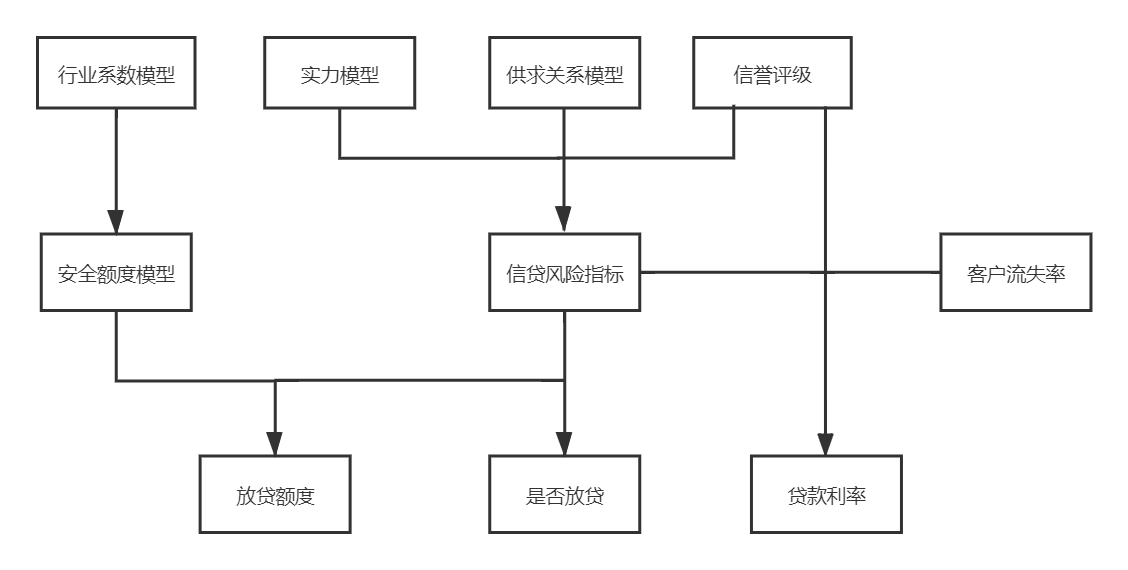
\includegraphics[width=.7\textwidth]{procedure1.jpg}
    \caption{问题一思路框图示意图}
    \label{fig:procedure1}
\end{figure}

\subsection{问题二的分析}
针对问题二,题目所给数据不同的地方在于附件二的302家企业没有人工评定的信誉评级,但由于我们在问题一中已经建立了一个较为完善的
信贷策略选择模型,我们可以适当给出企业的信誉评级。同时考虑到得到的安全额度可能不足达到银行贷款固定总额,因此应对安全额度进行调整,
采用正态分析法。整理相关数据,应用我们建立的银行选择决策模型,即可给出银行在年度信贷总额为 1 亿元时对这些企业的信贷策略。

\subsection{问题三的分析}
针对问题三,我们以新冠病毒疫情为例做出具体的分析,同时将该模型进行推广,可以运用到多数突发情况。具有普适性的,对于不同的
行业来说,新冠病毒疫情对于不同的行业影响力不一样,对于不同类别的企业来说,也有不同的影响。首先应考虑到其最显著的影响结果,
即对行业收入的影响,其间接地影响到信贷风险结果。国家政策\cite{liuqi2020}指出,金融机构应发挥对疫情防控工作和实体经济的
支持作用,因此除了银行的利润外,我们还应考虑到对困难企业的扶持。引进扶持优惠指标对受疫情负影响较大的企业进行扶持,综上得出
信贷调整策略。

\section{模型的假设与符号说明}
\subsection{符号说明}
\begin{table}[H]
    \centering
    \caption{符号说明}\label{tab:001}
    \rowcolors{1}{white}{Lavender}
    \begin{tabular}{ccc||ccc}
        {\bf 符号} & {\bf 含义} & {\bf 单位} & {\bf 符号} & {\bf 含义} & {\bf 单位} \\
        $m_i$ & 企业每条进项发票的价税合计 & 元 &$m_e$ & 企业每条销项发票的价税合计 & 元 \\
        $y$ & 银行总盈利 & 元 & $p$ & 企业利润率 & \\
        $ip$ & 企业平均年利润增长率 &  & $T$ & 企业最近一年的年收入 & 元\\
        $G$ & 企业信誉评级 & & $c$ & 企业信贷风险值 & \\
        $n$ & 相应的有贷款资格的企业的数目 & 个 & $l$ & 企业贷款额度 &  元\\
        $R$ & 贷款额度相对应的基准利率 & & $r$ & 企业贷款利率 & \\
        $r_base$ & 对于某个贷款额度的银行利率 & & $r_d$ & 突发情况优惠扶持利率比 &\\
        $l_s$ & 企业安全贷款额度 & 元 & $l_m$ & 企业最大贷款额度 & 元\\
        $L$ & 银行年度信贷总额 & 元 & $\pi$ & 行业调整系数 &    \\
        $p$ & 贷款利率 & 元  & $w$ & 客户流失率 &  \\ 
        \hiderowcolors
    \end{tabular}
\end{table}

\subsection{基本假设}
(1) 假设一:假定附件所给发票数据为该时间范围内企业的全部交易发票数据。

(2) 假设二:银行年度信贷总额固定意味着在信贷策略中将该额度全部贷出。

(3) 假设三:默认总的贷款时间为贷款期限最大值,即1年。

\section{模型的建立与求解}
\subsection{问题一模型的建立与求解}
\subsubsection{决策影响因素及其影响机理的分析}
本问要求分析银行在固定年度信贷总额下的放贷一年的信贷策略,使收益较大,信贷策略包括是否为企业放贷以及贷款的额度和利率。计算出
各个企业的信贷风险指标,对其中信贷风险低的企业进行放贷。综合考虑客户流失率,对其中信誉好的企业给予利率优惠。

进一步分析这些因素,可以发现信贷风险指标主要由:实力、供求关系以及信誉评级三个根本要素决定。其中,实力由利润率、平均年利润
增长率以及上下游企业的影响力决定;分析进方和销方的单位数量、稳定的进销方占比以及作废发票和负数发票占比可以判断供求关系的稳定性。

由此得到如图\ref{fig:procedure1}所示的影响信贷风险因素的指标及其影响机理图:

\begin{figure}[H]
    \centering
    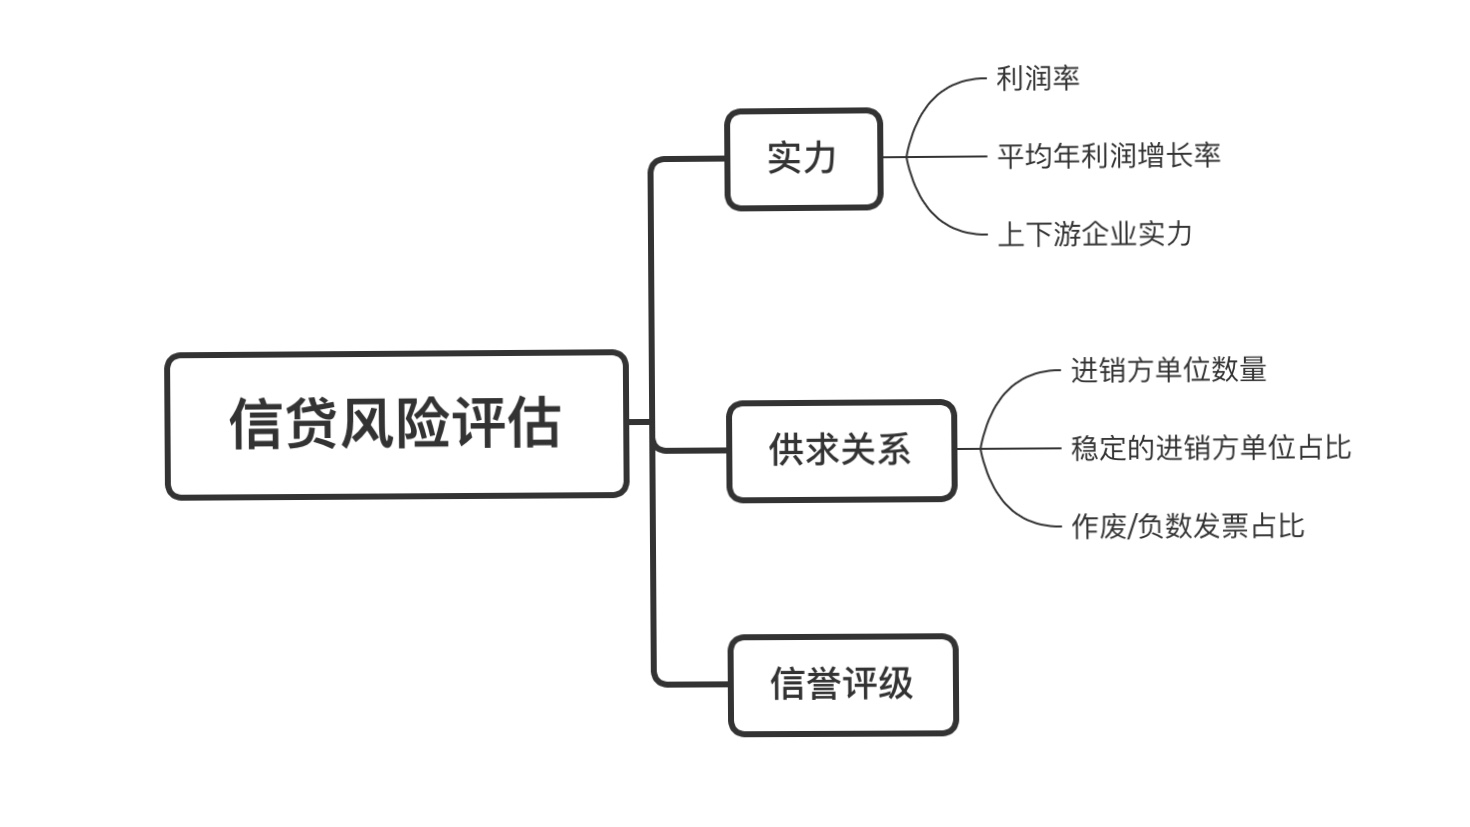
\includegraphics[width=.8\textwidth]{procedure .jpg}
    \caption{信贷风险指标评估因素}
    \label{fig:procedure}
\end{figure}

利润率和年利润平均增长率代表着该企业的盈利当前状况和企业盈利发展状况;通过判断进销商与所给数据中企业合作的数量来判断其影响
力,即该企业上下游的影响力。而进销方数量象征着进货和销售渠道的广泛度;而有与之合作稳定的进销方代表其有稳定的进货和销售渠道,
与广泛性同等重要;附件数据中有部分发票是作废发票,代表着为交易活动开具发票后,因故取消了该项交易;还有部分发票是负数发票,
代表着在为交易活动开具发票,企业已入账记税后,购方因故发生退货并退款的情况,除了正常处理的情况,若这两类发票在发票总数中
占比异常,可能代表着企业有逃税或做假账的嫌疑,影响企业供求关系稳定性。

值得注意的是,对于放贷额度$l$,各行业不同的贷款指标应纳入考虑,即不同的行业在贷款额度上应有所不同。根据第三方平台中纳税
申报的数据\cite{dangxinlu2016}作为依据得出行业的调整系数$\pi$:
\begin{table}[!htbp]
    \caption{行业调整系数}\label{tab:002} \centering
    \setlength{\tabcolsep}{13mm}{    %按页面宽度调整表格
    \begin{tabular}{ccc}
        \toprule[1.5pt]
        行业编号 & 行业类别 & 行业系数$\pi$ \\
        \midrule[1pt]
        1 & 农林牧渔业 & 35.71\%\\
        2 & 工业 & 31.25\%\\
        3 & 建筑业 & 50.00\%\\
        4 & 交通运输、仓储及邮政业 & 58.82\%\\
        5 & 信息技术服务业 & 20.41\%\\
        6 & 批发和零售贸易业 & 14.29\%\\
        7 & 住宿和餐饮业 & 25.00\%\\
        8 & 房地产业 & 166.67\%\\
        9 & 社会服务业 & 66.67\%\\
        10 & 传播与文化业 & 50.00\%\\
        \bottomrule[1.5pt]
    \end{tabular}}
\end{table}

\subsubsection{信贷风险评价模型}
本问题中最为关键的部分就是建立信贷风险评估模型,其分为三个部分:

    \textbf{1) 实力模型}
    
    实力模型由 3 个因素决定,包括上游企业影响力和下游企业影响力,利润率以及平均年利润增长率。

    上游企业指的是提供原材料和零部件制造和生产的行业,在本题中默认为进货方;下游企业指处在整个产业链的末端,加工原材料和零
    部件,制造成品和从事生产的产业,在本题中默认为销出方。上下游企业的影响力可以间接作为判断该企业影响力的依据之一。通过
    Excel软件和Python程序分析出123个企业对应的进销商以及各个进销商与123个企业中进行交易的企业数目,以该数据作为判断上下游
    企业影响力的标准,划分影响力较大和影响力较小的两类上下游企业,判断出与影响力大的上下游企业的交易数目及稳定性。

    利润率$p$表示为:
    \begin{equation}
        p = \frac{\sum_{n = 1}^{n_2} m_e - \sum_{n = 1}^{n_1}m_i}{\sum_{n=1}^{n_2}m_e}   
    \end{equation}
    
    其中$m_i$表示对于某一企业的一条进项价税总和,$m_e$表示对于该企业的一条销项价税总和,而$n_1$表示该企业进项发票的数目,
    $n_2$表示该企业销项发票的数目。
    
    平均年利润增长率$ip$表示均衡计算企业的近几年平均利润增长水平,从而客观评价企业的发展能
    力状况,由于给定数据中部分企业的发票时限并不完整,对于某些发票时间范围少于一年的,默认其利润增长率为0;对于部分进项与
    销项时间不对应的数据,仅选择重叠时间部分做运算。

    得出以上三个指标后,引入层次分析法\upcite{chenyihua1997}得出综合实力值,根据各因素的重要性关系建立实力判断矩阵,求得
    相应权值结果:
    \begin{table}[!htbp]
        \caption{实力判断矩阵}\label{tab:003} 
        \raggedleft
        \begin{tabular}{cccccc}
            \toprule[1.5pt]
             & 上游影响力 & 下游影响力 & 销售利润 & 平均利润年增长率 & 权值$\omega$\\
            \midrule[1pt]
            上游影响力 & 1 & 1 & 1/3 & 1/5 & 0.098 93\\
            下游影响力 & 1 & 1 & 1/3 & 1/5 & 0.098 93\\
            销售利润 & 3 & 3 & 1 & 1/2 & 0.283 85\\
            平均利润年增长率 & 5 & 5 & 2 & 1 & 0.518 30\\
            \bottomrule[1.5pt]
        \end{tabular}
    \end{table}

    \textbf{2) 供求关系模型}

    供求关系是否稳定是判断产业发展状况的重要指标之一。
    若其进销方单位数量多,则证明其原料来源和产品销路广泛,渠道众多;稳定的进销方是衡量企业供求关系稳定的重要指标之一,用稳定
    的进销方在总的交易单位中的比值来表示;而作废发票和负数发票的开具,除了正常的开具错误、销货退回等原因,还有可能是企业恶意
    隐瞒收入,虚开发票,销售方与接票方恶意串通达到偷税目的的表现。因此我们需要判断作废发票和负数发票在总发票数中的占比,若
    有异常情况,应影响其信誉度。

    \begin{table}[H]
        \caption{供求关系判断矩阵}\label{tab:004} 
        \raggedright
        \begin{tabular}{lccccl}
            \toprule[1.5pt]
             & 作废发票占比 & 进销方数量 & 稳定进销方占比 & 负数发票占比 & 权值$\omega$ \\
            \midrule[1pt]
            作废发票占比 & 1 & 1/5 & 1/3 & 1 & 0.095 45\\
            进销方数量 & 5 & 1 & 3 & 5 & 0.559 60\\
            稳定进销方占比 & 3 & 1/3 & 1 & 3 & 0.249 50\\
            负数发票占比 & 1 & 1/5 & 1/3 & 1 & 0.095 50\\
            \bottomrule[1.5pt]
        \end{tabular}
    \end{table}

    \textbf{3) 信贷风险评价模型}

    根据上面讨论的两个模型,我们可以求得各企业的实力值和供求关系稳定值。综合银行内部评定的信誉等级,可以量化求解出最终的
    信贷风险。同样利用层次分析法,根据各个因素的重要性得到判断矩阵并求出相应的权值:

    \begin{table}[!htbp]
        \caption{信贷风险指标判断矩阵}\label{tab:005} 
        \centering
        \setlength{\tabcolsep}{10mm}{    %按页面宽度调整表格
        \begin{tabular}{ccccc}
            \toprule[1.5pt]
             & 实力 & 供求关系 & 信誉评级 & 权值$\omega$ \\
            \midrule[1pt]
            实力 & 1 & 5 & 3 & 0.648 33\\
            供求关系 & 1/5 & 1 & 1/2 & 0.122 02\\
            信誉评级 & 1/3 & 2 & 1 & 0.229 65\\
            \bottomrule[1.5pt]
        \end{tabular}}
    \end{table}

    由于不考虑信誉等级为D级的,共24家企业,则最终需要计算99家企业的信贷风险,将其指标值量化到$[0, 1]$区间得到各个企业的信贷风险
    结果,其散点图表示为:

    \begin{figure}[H]
        \centering
        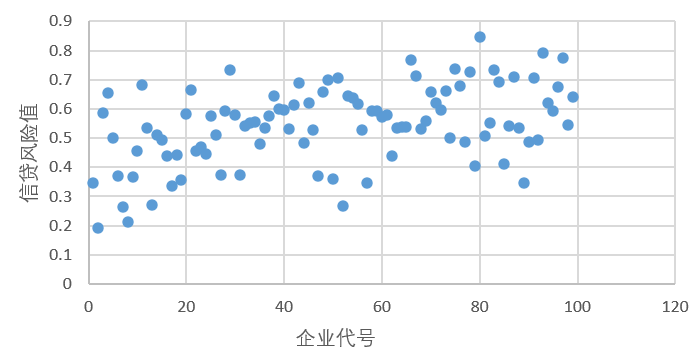
\includegraphics[width=.7\textwidth]{reliability.png}
        \caption{信贷风险指标评估因素}
        \label{fig:reliability}
    \end{figure}

\subsubsection{安全额度模型}
得到各企业的信贷风险指标后,可以筛选出信贷风险较小的企业作为放贷对象。接着,我们需要得到贷款额度,这里引入安全贷款额度,
以表示当小于或等于该贷款额度时,风险是处于可掌控范围内的。根据行业的不同特点,采用最近一年的年收入$T$作为企业贷款的基础
指标,表示近期一段时间内企业的收入情况,能够充分反映企业的经营状况优劣。以行业调整系数$\pi$作为贷款安全额度的单一财务指标,
可将贷款安全额度$l_s$表示为:
\begin{equation}
    l_s = \pi\times T_i  
\end{equation}

值得注意的是,得到安全额度后我们应根据固定的银行年度信贷总额将其映射到$10-100$万区间以内,考虑到当银行把全部金额贷出时得到
的利润相对最大。参考\cite{dangxinlu2016}基于层次法对贷款额度和信贷风险的分析,判断当贷款额度增加到安全额度的 1.2 倍,
1.5倍,2 倍时,信贷风险是否超过设定阈值$c$,求解出贷款额度能在安全额度基础上扩充的最大倍数。最终我们可获得各企业的贷款
额度$l$的区间,即其安全额度$l_s$至最大贷款额度$l_m$。

\subsubsection{决策模型的建立与银行决策的确定}
综合以上可给出放贷策略:

(1) 是否放贷

信贷风险的阈值设定参考信誉评级,在附件数据中,信誉评级为D等的企业占比约为$20\%$,因此,选择信贷风险值后$80\%$可进行贷款,
同时以前$20\%$信贷风险中最小的值为阈值$C$,即信贷风险高于$0.662\ 58$的企业认为是信贷风险较高的企业,不予以贷款。
采用$0-1$变量$Q$表征银行是否进行贷款的方案。若$Q_i$取 1,代表对该企业进行放贷,若$Q_i$取0则不予以贷款,表示为:
\begin{equation}
    Q_i = \begin{cases}
        1, &\text{如果} l = l_m \text{时,}c_i > C;\\
        0, &\text{如果 } l = l_m \text{时,}c_i \leqslant C;\\
    \end{cases}
\end{equation}
最终确定共有79家企业可以获得放贷,即 $a = 79$,剩余42家企业中有24家企业由于信誉评级为D级被筛除,另外18家企业属于信贷风险较高的企业。

(2) 目标函数及约束条件确立

目标函数为对利润$Z$求取最大值:
\begin{equation}
    max\ Z = \sum_{i=1}^{79}l_i \times r_i \times (1-w_i)
\end{equation}

其约束条件为:
\begin{equation}
    \begin{cases}
        & \sum_{i=1}^{79}l_i = L \\
        & 10 \leqslant l_i \leqslant l_m \\
    \end{cases}
\end{equation}

其中$l_i$指的是该企业的贷款额度,$l_i$需要满足两个条件,首先各个放贷企业的贷款额度之和应小于银行年度信贷总额,其次每个
企业的信贷额度还应在10万元和最大信贷额度$l_m$区间内。值得注意的是,可能会出现当各企业都取得最大信贷额度时仍没有满足银行
年度信贷总额,即没有将所有贷款额贷出,引入指标平均贷款额度$a$:
\begin{equation}
    \centering
    \text{平均信贷额度}\ 
    a = 
    \text{银行年度信贷总额}\ 
    L \div
    \text{有贷款资格的企业数目}\ 
    n
\end{equation}

我们应考虑一个函数使得其近似服从正态分布,并以平均信贷额度为期望值,使得各企业申请的最大贷款额度之和能大于将银行信贷总额,并且
使较多的企业合理申请贷款额度。例如,当平均贷款额度$a$取55万元时,可得到部分企业贷款额度分布区间:

\begin{figure}[!h]
    \centering
    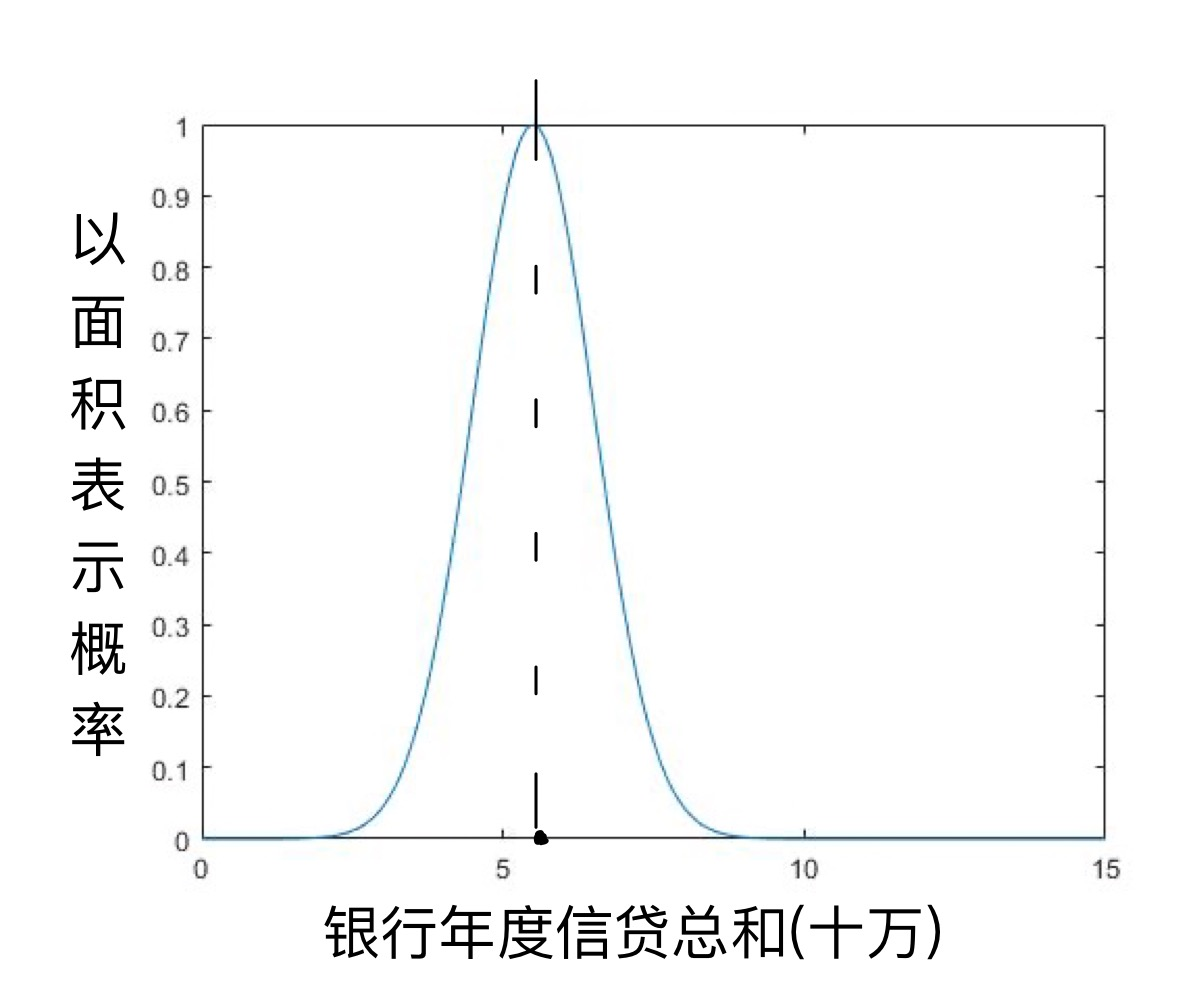
\includegraphics[width=.4\textwidth]{normal.jpg}
    % \caption{}
    \label{fig:normal}
\end{figure}

$r_i$指的是该企业的利率,我们认为贷款额度可以决定基准贷款利率
$r_{base}$,拟合出两者的线性函数关系,其中基准贷款利率映射到规定的$4\% - 15\%$区间:
\begin{equation}
    r_{base} = 0.00124\ l + 0.02633
\end{equation}

\begin{figure}[H]
    \centering
    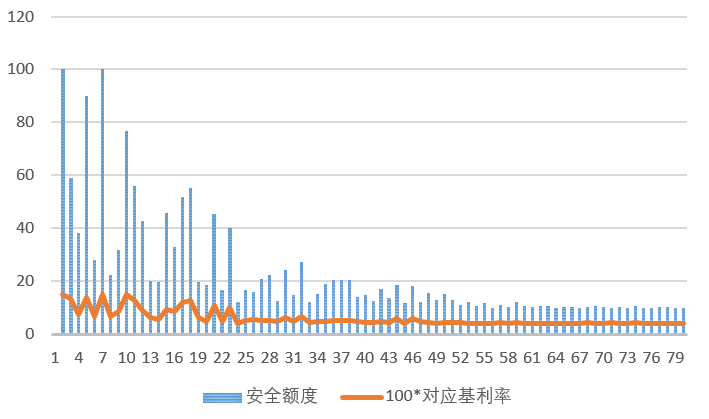
\includegraphics[width=.7\textwidth]{base_rate.png}
    \caption{贷款额度相对应的基利率}
    \label{fig:reliability}
\end{figure}

而对于某些信誉评级高,信贷风险小的企业来说,应有适当的利率优惠,信誉评级与信贷风险赋以相同的权重,并将优惠率映射到$[0.6, 1]$
区间,由于利率优惠不应过高,取最高优惠率阈值为 0.6,得到优惠率,乘以基准利率即可得到优惠后的利率$r_i$为:
\begin{equation}
    r_i = (-\frac{2}{5e-5} e^{0.5\times G_i + 0.5\times c_i} + \frac{5e-3}{5e-5}) \times r_{base}
\end{equation}

其中信誉与信贷风险的综合指标与优惠率的关系见下图:
\begin{figure}[H]
    \centering
    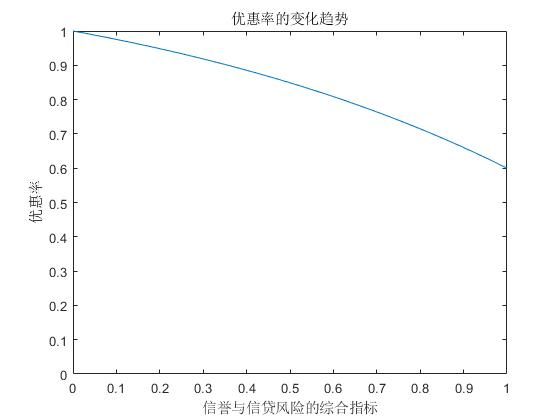
\includegraphics[width=.5\textwidth]{1.jpg}
    \caption{优惠率的变化趋势}
    \label{fig:reliability}
\end{figure}

$w_i$指的是相应利率和信誉评级下的客户流失率,根据附件三中所给的数据,可以拟合出在不同的利率下三种信誉评级的客户流失率:
\begin{equation}
    w_i = \begin{cases}
    7.524 r_i-0.0979,  &{\text{信誉评级为A时}};\\
    7.351 r_i-0.1178, &{\text{信誉评级为B时}};\\
    7.468 r_i-0.1379, &{\text{信誉评级为C时}};\\
    \end{cases}
\end{equation}

考虑当银行年度信贷总额足够大时,每个可贷款企业都可以选择其最大信贷额度,又由于贷款利率和相应的客户流失率都可以表示成贷款
额度的函数,实际上我们可以得到利润的最大值;而当银行年度信贷总额不足取得上述最大值时,我们将得到近似最大值,即相对最优的
银行信贷策略。

\subsection{问题二模型的建立与求解}
\subsubsection{模型建立}
根据不同的行业受不同的行业系数等其他因素影响,我们首先应该分析各个企业分别属于哪个行业,最终分析得到的柱形图显示:
\begin{figure}[H]
    \centering
    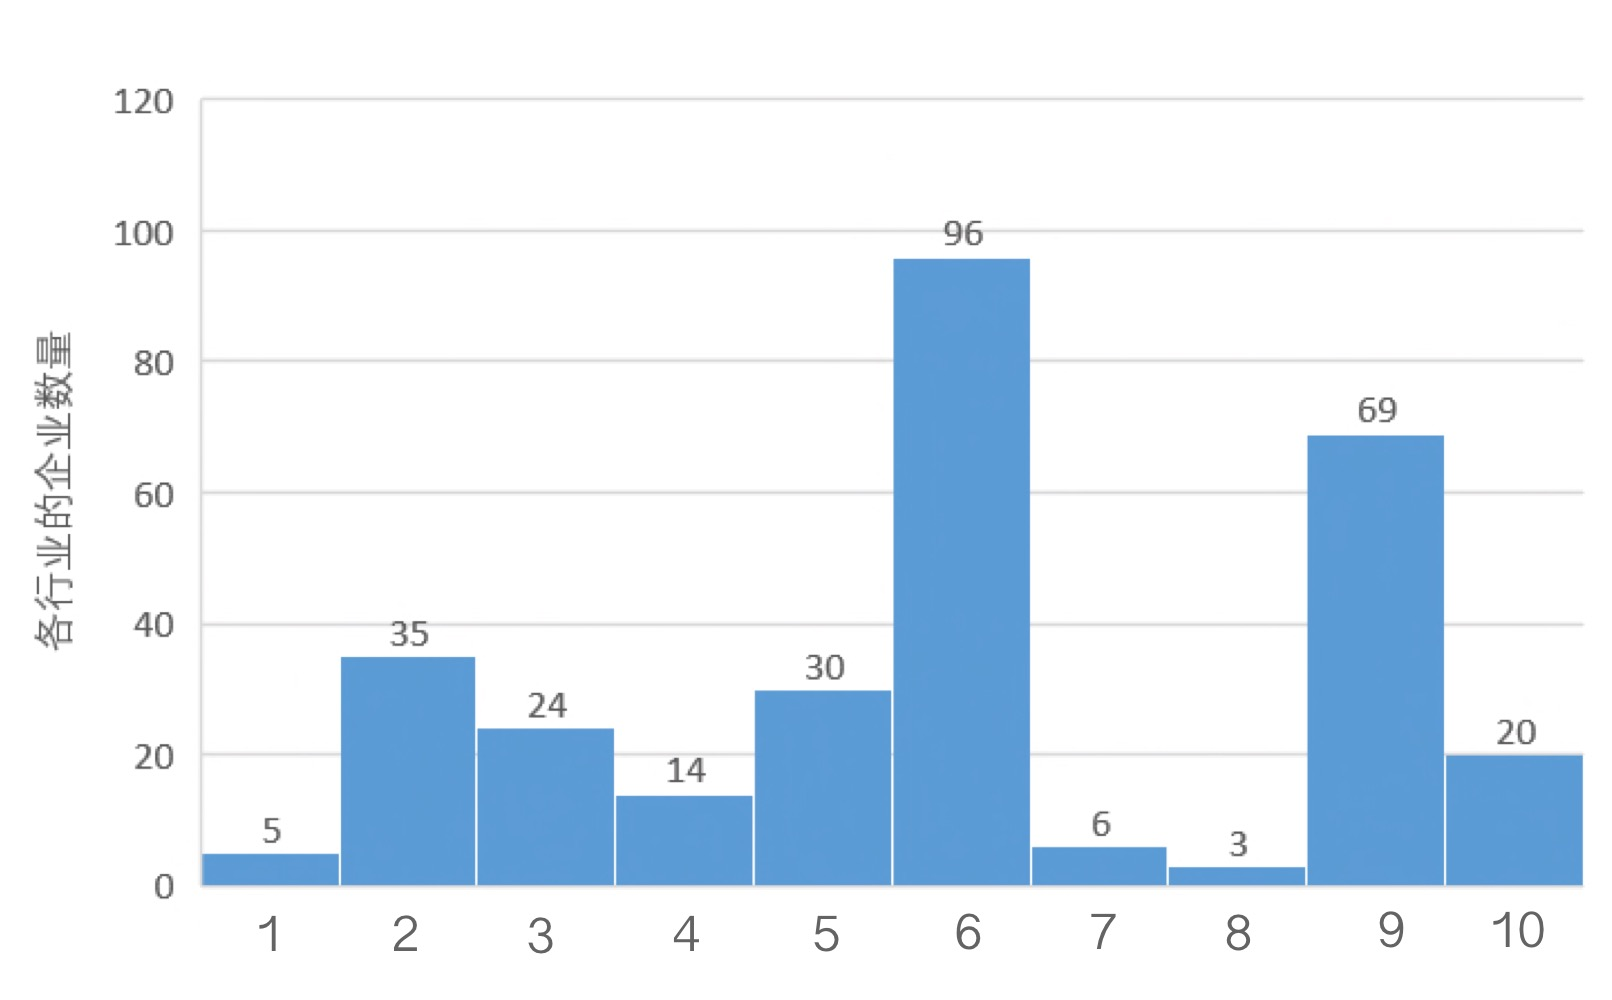
\includegraphics[width=.5\textwidth]{industry.jpg}
    \caption{各个行业所对应的企业个数}
    \label{fig:industry}
\end{figure}

由于本问题所给为302家无信贷记录企业的相关数据,因此我们需要对其信誉等级进行评估。而原信誉评级是由银行内部根据企业的实际
情况人工评定的,考虑到众多综合因素,无法仅通过发票信息进行判断,因此取附件A中信誉评级的众数,即B级作为302家企业的信誉评级。

应用问题一给出的信贷风险评估模型得出各个企业的信贷风险指标,并筛选信贷风险低于$0.662\ 58$的企业作为可放贷企业,共选择出242
个企业。

当银行年度信贷总额固定为 1 亿时,我们可以根据问题一中提到的贷款额度分布,正态化分析得到各企业的安全贷款额度,如图\ref{fig:zt},并利用安全
贷款额度模型判断其在信贷风险不超过阈值下的最大贷款额度,如图\ref{fig:zt2}:

\begin{figure}[H]
    \centering
    \begin{minipage}[c]{0.4\textwidth}
        \raggedright
        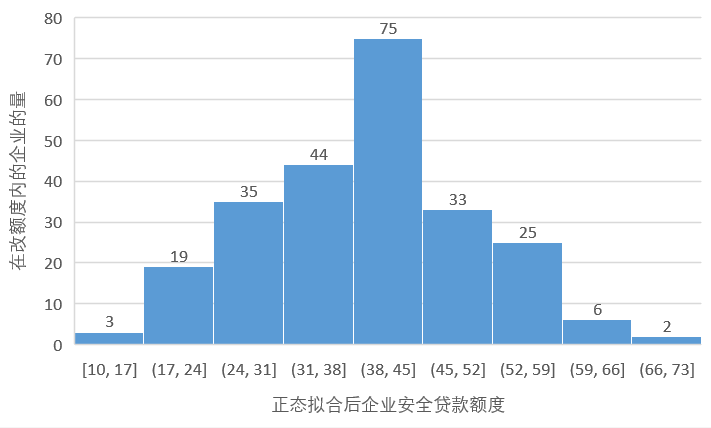
\includegraphics[width=1\textwidth]{zt.png}
        \subcaption{正态化后的安全贷款额度}
        \label{fig:zt}
    \end{minipage}
    \begin{minipage}[c]{0.4\textwidth}
        \raggedleft
        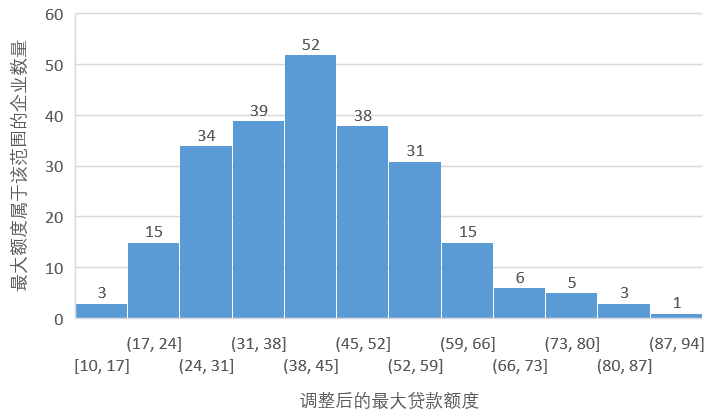
\includegraphics[width=1\textwidth]{zt2.png}
        \subcaption{最大贷款额度}
        \label{fig:zt2}
    \end{minipage}
    \caption{正态化的安全贷款额度模型}
    \label{fig:zt-figure}
\end{figure}

\subsubsection{模型求解结果}
目标函数为利润$Z$的最大值,可如上述表示为:
\begin{equation}
    max\ Z = \sum_{i=1}^{n=242}l_i \times r_i \times (1-w_i)
\end{equation}

最终求得的结果为:当银行年度信贷额度固定为 1 亿时,能达到最高的利润为$404\ 4248$元,同时也得到了各个企业的合理放贷额度和
相应的利率,得到最终的放贷策略。详细的信贷调整模型结果见支撑材料。


\subsection{问题三模型的建立与求解}
\subsubsection{新冠病毒疫情对各行业的影响}
新冠肺炎病毒的爆发攻陷了全国所有的省份,使所有人深陷病毒的困扰和与生命的抗争中,至2020年9月13日我国已累计确诊共90657人,
累计死亡人数共4741人,如图\ref{fig:reliability}显示了各地确诊人数统计情况,触目惊心:
\begin{figure}[!h]
    \centering
    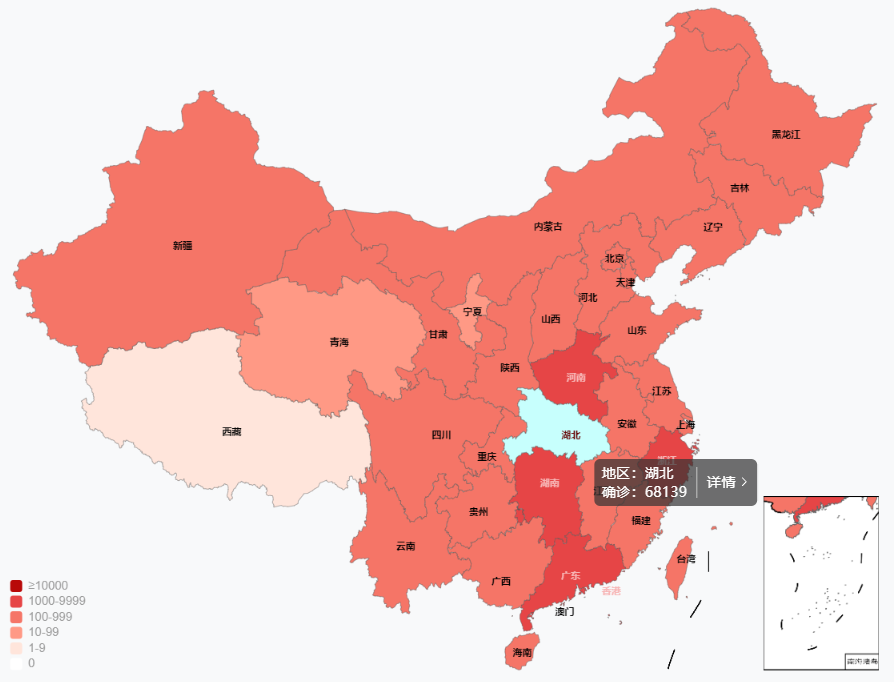
\includegraphics[width=.8\textwidth]{total.png}
    \caption{新冠疫情至2020年9月13日累计确诊人数\newline(数据来源自国家卫健委官方数据)}
    \label{fig:reliability}
\end{figure}

不仅如此,还对全国经济带来了巨大的冲击,其中这次疫情对中小微企业的影响更应受到我们的重视。由于其资金周转率较低,没有
充足的资金来源,抗市场压力能力较弱等特点,疫情发生后原材料无法及时送达,人员复工推迟等情况无法保证收入,而又面临着员工工资、
租金等刚性输出,中小微企业的生存面临着严峻的挑战。

朱武祥等人基于两次全国疫情冲击下中小微企业问卷调查的分析\cite{zhuwuxiang2020},显示总计58.05\%的受调查企业应收预计下降
20\%,超过$2/3$的企业资金维持能力不超过 2 个月,其中34\%的企业难以维持一个月。

而参考《新冠疫情对中国宏观经济的影响分析》\cite{mawanqing2020},我们可以得出下面的表格:
\begin{table}[H]
    \caption{受新冠疫情影响各行业的收入变化比例$\varphi$ }\label{tab:006}
    \centering
    \setlength{\tabcolsep}{13mm}{    %按页面宽度调整表格
    \begin{tabular}{ccc}
        \toprule[1.5pt]
        行业编号 & 行业类别 & 行业收入变化率$\varphi$  \\
        \midrule[1pt]
        1 & 农林牧渔业 & $-\ 3.2$\%\\
        2 & 工业 & $ -\ 9.6$\%\\
        3 & 建筑业 & $-17.1$\%\\
        4 & 交通运输、仓储及邮政业 & $-\ 1.5$\%\\
        5 & 信息技术服务业 & $+13.2\%$\\
        6 & 批发和零售贸易业 & $-\ 12$\%\\
        7 & 住宿和餐饮业 & $-44.3$\%\\
        8 & 房地产业 & $-37.53$\%\\
        9 & 社会服务业 & $-12.2\%$\\
        10 & 传播与文化业 & $+\ 1.9$\%\\                                                           
        \bottomrule[1.5pt]
    \end{tabular}}
\end{table}

\subsubsection{建立新冠疫情信贷策略调整}
从表\ref{tab:006}中可以得出,除了信息技术服务业和传播与文化业之外,其余多数企业都受到了一定程度的负向影响,这些行业的中小微
企业偿债能力或下降,财务实力和投资能力被削弱,需要外部资金支持来恢复经营。而据调查\cite{zhuwuxiang2020}显示,有22.0\%的
企业希望获得贷款,因此调整新冠疫情下信贷策略是亟待解决的问题。

而企业收入的变化作为实力模型的重要影响因素之一,显然会对企业的信贷风险产生影响。对于如信息技术服务业和传播与文化业,疫情对其
带来了正面影响,即使其收入有明显增加,导致这类企业的信贷风险降低,同时我们不需要对其有突发情况扶持;而对于其他企业来说,疫情
对其产生了负面影响,即使其收入有明显减少,导致这类企业的信贷风险增加。但在疫情这类突发情况下,银行不仅作为一个盈利集团,更需要
发挥其对于民生和实体经济稳定发展的支持作用,并采取措施支持疫情防控工作。因此我们可以对受疫情灾害较为严重的行业提供扶持优惠
政策,在一定程度上降低其贷款利率。因此我们引入突发情况利率优惠$r_d$。得到突发情况下利率$r_i$的新模型:
\begin{equation}
    r_i = (-\frac{2}{5e-5} e^{0.5\times G_i + 0.5\times c_i} + \frac{5e-3}{5e-5}) \times r_{base} \times r_d
\end{equation}

其中,$r_d$需要分类讨论:
\begin{equation}
    r_d = \begin{cases}
        1, &\text{如果突发情况对该行业没有负面影响};\\
        f(\varphi), &\text{如果突发情况对该行业有负面影响};\\
    \end{cases}
\end{equation}

其中$f(\varphi)$是通过将负的行业收入变化率进行归一化,结果图\ref{fig:variable}:
\begin{figure}[H]
    \centering
    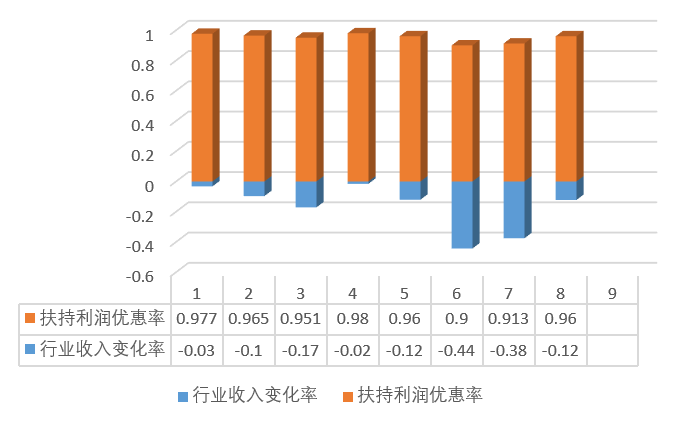
\includegraphics[width=.7\textwidth]{variable.png}
    \caption{行业收入变化率与扶持优惠利率的关系}
    \label{fig:variable}
\end{figure}

对于不同的企业类别,也有可能会对突发情况做出不同的反应。企业主要分类有:合资、独资、国有、私营、股份制、有限责任等等,
而对于中小微型企业个体经营、私营和有限责任公司占比较大,其中个体经营的风险承担率显然是更小的。

同时还应考虑到,由于信贷风险的变化,根据安全额度模型会造成最大贷款额度的变化,同时也会改变原定的利率及优惠政策,再综合考虑
扶持优惠利率,将得到一个针对疫情影响的信贷调整策略。详细的信贷调整模型结果见支撑材料。

\section{模型的优缺点}
\subsection{模型的优点}
(1)问题一基于层次分析法,在回答基本决策的基础上,进一步对较为完整的指标进行了考虑,架构清晰,增强实用性。

(2)问题二很好地结合了实际情况,实用性较强,对现实有很强的指导意义。

(3)问题三建立的调整策略能够应对大多数突发情况,在实际生活中有着重要作用,且模型较为新颖,结果合理。

\subsection{模型的缺点}
(1)对于模型的部分参数是通过实际情况进行估计的,对结果产生了一定的误差。

(2)问题二求得的解可能并非事实最优解,由于受计算机算力限制,存在近似误差。

(3)在问题三中由于可以作为支撑的数据材料较少,例如仅对企业的类别进行了定性分析,存在改进空间。

(4)默认所有贷款时间均为最大贷款期限1年,应深入分析不同的贷款期限对模型的影响。

\section{模型的推广与改进方向}
\subsection{模型的改进方向}
(1)详细调查时间范围内更完整的企业收支运行情况数据,使模型中的部分参数更精密。 

(2)基于更加详尽的数据建立更完善的影响因素对信贷决策的模型,使信贷策略更加完备。

\subsection{模型的推广}
(1)除了对于固定额度的银行年度贷款,还可以基于问题一构建的模型解决可调整额度的银行贷款策略。

(2)可以更加广泛地应用问题三建立的突发情况扶持利率优惠模型,针对突发状况及时进行调整。

%参考文献
\begin{thebibliography}{9}%宽度9
    \bibitem[1]{wangxiang2008}
    王翔. 
    \newblock 基于关系型贷款的大银行对小企业的贷款定价研究[D].
    \newblock 中南大学,2008.

    \bibitem[2]{lixinyang2012}
    李昕阳.
    \newblock 刍议以财务评价为核心的商业银行中小企业信用评级体系重构[J].
    \newblock 商业经济,2012(08):110-111+117.

    \bibitem[3]{liuqi2020}
    刘琪.
    \newblock 央行等五部门:进一步强化金融支持疫情防控工作  支持实体经济稳定发展[J].
    \newblock 中国中小企业,2020(03):30-31.

    \bibitem[4]{dangxinlu2016}
    党馨璐.
    \newblock 基于层次分析法的小微企业信用贷款风险评估研究[D].
    \newblock 山东财经大学,2016.

    \bibitem[5]{chenyihua1997}
    陈义华.
    \newblock 数学建模的层次分析法[J].
    \newblock 甘肃工业大学学报,1997(03):93-98.

    \bibitem[6]{zhuwuxiang2020}
    朱武祥,张平,李鹏飞,王子阳.
    \newblock 疫情冲击下中小微企业困境与政策效率提升——基于两次全国问卷调查的分析[J].
    \newblock 社会科学文摘,2020(06):5-7.

    \bibitem[7]{mawanqing2020}
    马琬清.
    \newblock 新冠疫情对中国宏观经济的影响分析[J].
    \newblock 湖北经济学院学报(人文社会科学版),2020,17(09):34-37.
\end{thebibliography}

\begin{appendices}
    \section{问题一:AHP.m}
    \begin{lstlisting}[language=matlab]
    function [Q]=AHP(B,x)
X = mapminmax(x', 0.02, 0.98);
%Q为权值,B为对比矩阵
%导入判别矩阵B
[n,m]=size(B);
%判别矩阵具有完全一致性
for i=1:n
    for j=1:n
        if B(i,j)*B(j,i)~=1   
        fprintf('i=%d,j=%d,B(i,j)=%d,B(j,i)=%d\n',i,j,B(i,j),B(j,i))  
        end  
    end
end
%求特征值特征向量,找到最大特征值对应的特征向量
[V,D]=eig(B);
tz=max(D);
tzz=max(tz);
c1=find(D(1,:)==max(tz));
tzx=V(:,c1);%特征向量
%权
quan=zeros(n,1);
for i=1:n
quan(i,1)=tzx(i,1)/sum(tzx);
end
Q=quan;
Q
%一致性检验
CI=(tzz-n)/(n-1);
RI=[0,0,0.58,0.9,1.12,1.24,1.32,1.41,1.45,1.49,1.52,1.54,1.56,1.58,1.59];
%判断是否通过一致性检验
CR=CI/RI(1,n);
if CR>=0.1
   fprintf('没有通过一致性检验\n');
else
  fprintf('通过一致性检验\n');
end
Q=Q'*X;
end
\end{lstlisting}

\section{问题一:AHP1.m}
\begin{lstlisting}[language=matlab]
    function f = fun2(l)
    [X,textdata]=xlsread('风险分析及额度设置.xlsx');
    k = X(:,4:4);
    f=l;
    [n,m]=size(k);
    rate = fun1(l);
    for i=1:n
        m = rate(i:i,:);
        if k(i:i,:)==0.25
            %f(i:i,:) = 504.7*m^3-207.4*m^2+32.16*m-0.9735;
            f(i:i,:) = 7.468*m-0.1379;
        elseif k(i:i,:)==0.5
            %f(i:i,:) = 552.8*m^3-225.1*m^2+33.99*m-1.017;
            f(i:i,:) = 7.351*m-0.1178;
        else
            %f(i:i,:) = 640.9*m^3-258.6*m^2+37.97*m-1.121;
            f(i:i,:) = 7.524*m-0.09793;
        end
    end
\end{lstlisting}  

\section{问题一:AHPrelation.m}
\begin{lstlisting}[language=matlab]
    [X,textdata]=xlsread('供求关系源数据.xlsx');
    x=X(:,2:5);
    A1=[1,1/5,1/3,1;
        5,1,3,5;
        3,1/3,1,3;
        1,1/5,1/3,1;];
    Q1=AHP(A1,x);
    A2=[1,1/5,1/3,1;
        5,1,3,5;
        3,1/3,1,3;
        1,1/5,1/3,1;];
    x=X(:,6:9);
    Q2=AHP(A2,x);
    x=[Q1;Q2]';
    Q3=AHP1(x);
\end{lstlisting}

\section{问题一:AHPrisk.m}
\begin{lstlisting}[language=matlab]
    [X,textdata]=xlsread('风险评估.xlsx');
x=X(:,2:4);
A1=[1,5,3;
    1/5,1,1/2;
    1/3,2,1;];
Q1=AHP(A1,x);
\end{lstlisting}

\section{问题一:AHPstrength.m}
\begin{lstlisting}[language=matlab]
[X,textdata]=xlsread('实力评价源数据.xlsx');
x=X(:,1:4);
A1=[1,1,1/3,1/5;
    1,1,1/3,1/5;
    3,3,1,1/2;
    5,5,2,1;];
Qs=AHP(A1,x);
\end{lstlisting}

\section{问题一:fun1.m}
\begin{lstlisting}[language=matlab]
    function f = fun1(l)
f = 0.00124*l+0.02633;
[X,textdata]=xlsread('风险分析及额度设置.xlsx');
x = X(:,5:5);
x1 = mapminmax(x', 0, 1);
x = X(:,4:4);
x2 = mapminmax(x', 0, 1);
x3 = 0.5*x1+0.5*x2;
x3 = mapminmax(x3, 0, 1);
y = -2/(5*exp(1)-5)*exp(x3)+(5*exp(1)-3)/(5*exp(1)-5);
f = y.*f';
[n,m]=size(f);
for i=1:m
    if(f(:,i:i)<0.04)
        f(:,i:i)=0.04;
    end
end
f=f';
\end{lstlisting}

\section{问题一:fun2.m}
\begin{lstlisting}[language=matlab]
    function f = fun2(l)
[X,textdata]=xlsread('风险分析及额度设置.xlsx');
k = X(:,4:4);
f=l;
[n,m]=size(k);
rate = fun1(l);
for i=1:n
    m = rate(i:i,:);
    if k(i:i,:)==0.25
        %f(i:i,:) = 504.7*m^3-207.4*m^2+32.16*m-0.9735;
        f(i:i,:) = 7.468*m-0.1379;
    elseif k(i:i,:)==0.5
        %f(i:i,:) = 552.8*m^3-225.1*m^2+33.99*m-1.017;
        f(i:i,:) = 7.351*m-0.1178;
    else
        %f(i:i,:) = 640.9*m^3-258.6*m^2+37.97*m-1.121;
        f(i:i,:) = 7.524*m-0.09793;
    end
end
\end{lstlisting}

\section{问题一:fun3.m}
\begin{lstlisting}[language=matlab]
function f = fun3(l)
k = l.*fun1(l).*(1-fun2(l));
[n,m] = size(l);
f=0;
for i=1:n
    f = f+k(i:i,:);
end
f=-f;
\end{lstlisting}

\section{问题一:test.m}
\begin{lstlisting}[language=matlab]
[X,textdata]=xlsread('风险分析及额度设置.xlsx');
x = X(:,9:9);
[l,y] = fmincon('fun3',rand(79,1),[],[],ones(1,79),10,0.1.*ones(79,1),0.01.*x)
\end{lstlisting}

\section{问题一:软件操作过程}
\begin{lstlisting}
    一.附件一数据处理
1.有效数据修正:
	1>筛选并删除作废发票项
    2>将E14,E45对应的文本数值转换为数字格式(通过设置一个值为1的单元格,复制,选中文本数值的单元格,
    右键选择性粘贴,选择乘法)
2.负数数据统计(或者先计算正数发票数量,再用总有效数量减):
	1>有效数据修正(如1)
	2>筛选并删除金额为正的项
	3>建立数据透视表,筛选企业代号与金额计数来统计各企业进项与销项的负向发票数
3.销售利润率计算:
	1>有效数据修正(如1)
    2>分别为进项、销项发票信息建立数据透视表,计算每个企业的进项价税合计的总
    和与销项价税合计的总和,并由此计算出销售利润率
4.平均年利润增长率:
	1>有效数据修正(如1)
    2>分别为进项、销项发票信息建立数据透视表,显示每一年的进项价税合计的值与销项价税合计
    的值,由所显示的进项和销项的年份情况,选择性删除
    只有进项没有销项
      或者只有销项没有进项的年份的数据(该部分主要是2016年和2020年的部分月份,不能代表全
      年的情况)由此计算每一年的利润,并据此计算
      每一年的利润增长率,
	  最后计算平均年利润增长率。
5.近一年收入:
	1>有效数据修正(如1)
    2>建立销项发票信息的数据透视表,显示每一年的收入情况,统计2019年的收入,如果没有假定选
    用2018年的数据(极少数)。
6.有效发票计数
	1>有效数据修正(如1)
	2>建立销项发票信息的数据透视表,显示每一个企业的总发票数,即有效发票总数。
7.作废发票计数
	1>根据原附件数据建立数据透视表,显示每一个企业的总发票数,即所有发票数;
	2>用所有的发票数减去有效的发票数即为作废发票数。
二.附件二数据处理
	excel操作类似附件一的数据处理
三.matlab命令:
1.计算企业可靠性的归一化值:
	1.输入除去信誉为D的企业,其他企业的可靠性值x;
	2.输入命令:x1 = mapminmax(x', 0, 1);(得到归一化值)
	3.输入命令:x1 = x1'(转化为一列数据)
\end{lstlisting}

\section{问题二:zhengtai.m}
\begin{lstlisting}[language=matlab]
    mu=4.13;
p0=0;
l=0;
p1=0;
x1=[];
x2=[];
x3=[];
x4=[];
x5=[];
x6=[];
x7=[];
x8=[];
x9=[];
[X,textdata]=xlsread('乘行业系数后的值及对应的正态分布映射.xlsx');
x=X(:,2:2);
[n,m]=size(x);
p1 = normcdf(10,mu,1)-normcdf(9,mu,1)
for j=1:n
    if j/242<p1
        x9=[x9,x(j:j,:)];
    elseif j/242>=p1
        l=j;
        break;
    end
end
p0=p1;
p1 = normcdf(10,mu,1)-normcdf(8,mu,1)
for j=l:n
    if j/242<p1
        x8=[x8,x(j:j,:)];
    elseif j/242>=p1
        l=j;
        break;
    end
end
p0=p1;
p1 = normcdf(10,mu,1)-normcdf(7,mu,1)
for j=l:n
    if j/242<p1
        x7=[x7,x(j:j,:)];
    elseif j/242>=p1
        l=j;
        break;
    end
end
p0=p1;
p1 = normcdf(10,mu,1)-normcdf(6,mu,1)
for j=l:n
    if j/242<p1
        x6=[x6,x(j:j,:)];
    elseif j/242>=p1
        l=j;
        break;
    end
end
p0=p1;
p1 = normcdf(10,mu,1)-normcdf(5,mu,1)
for j=l:n
    if j/242<p1
        x5=[x5,x(j:j,:)];
    elseif j/242>=p1
        l=j;
        break;
    end
end
p0=p1;
p1 = normcdf(10,mu,1)-normcdf(4,mu,1);
for j=l:n
    if j/242<p1
        x4=[x4,x(j:j,:)];
    elseif j/242>=p1
        l=j;
        break;
    end
end
p0=p1;
p1 = normcdf(10,mu,1)-normcdf(3,mu,1);
for j=l:n
    if j/242<p1
        x3=[x3,x(j:j,:)];
    elseif j/242>=p1
        l=j;
        break;
    end
end
p0=p1;
p1 = normcdf(10,mu,1)-normcdf(2,mu,1);
for j=l:n
    if j/242<p1
        x2=[x2,x(j:j,:)];
    elseif j/242>=p1
        l=j;
        break;
    end
end
p0=p1;
p1 = normcdf(10,mu,1)-normcdf(1,mu,1);
for j=l:n
    if j/242<p1
        x1=[x1,x(j:j,:)];
    elseif j/242>=p1
        l=j;
        break;
    end
end
x1=[x1,x(l:l,:)];
x1=mapminmax(x1, 0.1, 0.2);
x2=mapminmax(x2, 0.2, 0.3);
x3=mapminmax(x3, 0.3, 0.4);
x4=mapminmax(x4, 0.4, 0.5);
x5=mapminmax(x5, 0.5, 0.6);
x6=mapminmax(x6, 0.6, 0.7);
last = [x1,x2,x3,x4,x5,x6]*100;
last = last';
\end{lstlisting}


\section{model.py}
\begin{lstlisting}[language=python]
# 出项或销项单位影响力.py
import openpyxl
import xlrd

# 该文件代码用于统计出项或销项单位影响力

def read_and_process_excel(bookname, sheetname):
    wb = xlrd.open_workbook(bookname)
    sheet = wb.sheet_by_name(sheetname)
    multilist = [[] * 1 for row in range(41551)]
    for i in range(1, sheet.nrows):
        company = sheet.cell(i, 3).value[1:]
        C = int(company)
        multilist[C].append(sheet.cell(i, 0).value)
    outwb = openpyxl.Workbook()  # 打开一个将写的文件
    outws = outwb.create_sheet(index=0)  # 在将写的文件创建sheet
    outws.cell(1, 1).value = '单位代号'
    outws.cell(1, 2).value = '合作企业数'
    for i in range(1, 31162):
        myset = set(multilist[i])
        outws.cell(i+1, 1).value = "D"+str(i).zfill(5)
        outws.cell(i+1, 2).value = len(list(myset))
    saveExcel = "2_单位影响力-销项.xlsx"
    outwb.save(saveExcel)  # 一定要记得保存

if __name__ == '__main__':
    read_and_process_excel('a.xlsx', '销项发票信息')


行业收入率变化映射.py
import xlrd
import xlwt
# 该文件代码用于映射某一行业的收入率变化

def read_and_process_excel(bookname, sheetname):
    wb = xlrd.open_workbook(bookname)
    sheet = wb.sheet_by_name(sheetname)
    lis = [-0.032,-0.096,-0.171,-0.015,0.132,-0.12,-0.443,-0.3753,-0.122,0.019]
    book = xlwt.Workbook(encoding='utf-8', style_compression=0)
    sheet1 = book.add_sheet('Sheet1', cell_overwrite_ok=True)
    for i in range(1, sheet.nrows):
        company = sheet.cell(i, 2).value
        C = int(company)
        sheet1.write(i, 3, lis[C-1])
    book.save("111.xls")
if __name__ == '__main__':
    read_and_process_excel('行业分类.xlsx', 'Sheet1')

计算安全额度.py
import xlrd
import xlwt
# 该代码用于计算某一行业的未映射如区间[10万,100万]的安全额度
def read_and_process_excel(bookname, sheetname):
    wb = xlrd.open_workbook(bookname)
    sheet = wb.sheet_by_name(sheetname)
    lis = [0.3571,0.3125,0.5,0.5882,0.2041,0.1429,0.25,1.6667,0.6667,0.5]
    book = xlwt.Workbook(encoding='utf-8', style_compression=0)
    sheet1 = book.add_sheet('Sheet1', cell_overwrite_ok=True)

    for i in range(0, sheet.nrows):
        print(sheet.cell(i, 1).value)
        print(1+float(sheet.cell(i, 3).value))
        a = sheet.cell(i, 1).value*lis[int(sheet.cell(i, 2).value-1)]*(1+float(sheet.cell(i, 3).value))
        # sum+=a
        sheet1.write(i,0,a)

    # junzhi = sum/(sheet.nrows-1)
    # miu = 100000000/(sheet.nrows-1)
    # bilv = junzhi/miu
    # a = 90/(72774785.1777869-693.689473)
    # b = miu-a*junzhi
    # for i in range(0, sheet.nrows-1):
    #     b = (90/cha)*(a-950.632247)+50
    #     sheet1.write(i+1,0,str(int(sheet.cell(i+1, 0).value)))
        # print(sheet.cell(i+1, 9).value)
        # sheet1.write(i+1,1,a*sheet.cell(i+1, 9).value+b)
        # sheet1.write(i, 1, b)
    book.save('124.xls')

if __name__ == '__main__':
    read_and_process_excel('近一年销售额.xlsx', 'Sheet1')

企业进项影响力统计.py
import xlrd
import xlwt
# 该文件代码用于统计某一企业的进项影响力

def read_and_process_excel(bookname, sheetname):
    wb = xlrd.open_workbook(bookname)
    sheet = wb.sheet_by_name(sheetname)
    #lis = ['A01205','A02382','A03310','A07368','A02282','A06204','A09920','A13655','A13116',
    'A03889','A05891','A13557','A07313','A13197','A03624','A06470','A03626','A00370','A07242']
    lis = ['C07715','C02374','C12006','C22413','C11143','C08135','C13284','C17386','C23259',
    'C13349','C07712','C23112','C22547','C11641','C13620','C05698','C05866','C11851','C07293']
    multilist = [[] * 1 for row in range(303)]
    for i in range(1, sheet.nrows):
        company = sheet.cell(i, 0).value[1:]
        C = int(company)-123
        multilist[C].append(sheet.cell(i, 3).value)
    book = xlwt.Workbook(encoding='utf-8', style_compression=0)
    sheet1 = book.add_sheet('Sheet1', cell_overwrite_ok=True)
    sheet1.write(0, 0, "企业代号")
    sheet1.write(0, 1, "影响力")
    for i in range(1, 303):
        sum = 0
        myset = set(multilist[i])
        for item in myset:
            if(str(item) in lis):
                sum+=1
        sheet1.write(i,0,"E"+str(i+123))
        sheet1.write(i,1,sum)
    book.save('2_企业影响力-进项.xls')

if __name__ == '__main__':
    read_and_process_excel('a.xlsx', '进项发票信息')

企业销项影响力统计.py
import xlrd
import xlwt
# 该文件代码用于统计某一企业销项影响力

def read_and_process_excel(bookname, sheetname):
    wb = xlrd.open_workbook(bookname)
    sheet = wb.sheet_by_name(sheetname)
    #lis = ['B08713','B03518','B08742','B03531','B08774']
    lis = ['D14951','D08689','D08718','D15038','D15257','D02772','D08821']
    multilist = [[] * 1 for row in range(303)]
    for i in range(1, sheet.nrows):
        company = sheet.cell(i, 0).value[1:]
        C = int(company)-123
        multilist[C].append(sheet.cell(i, 3).value)
    book = xlwt.Workbook(encoding='utf-8', style_compression=0)
    sheet1 = book.add_sheet('Sheet1', cell_overwrite_ok=True)
    sheet1.write(0, 0, "企业代号")
    sheet1.write(0, 1, "影响力")
    for i in range(1, 303):
        sum = 0
        myset = set(multilist[i])
        for item in myset:
            if(str(item) in lis):
                sum+=1
        sheet1.write(i,0,"E"+str(i+123))
        sheet1.write(i,1,sum)
    book.save('2_企业影响力-销项.xls')

if __name__ == '__main__':
    read_and_process_excel('a.xlsx', '销项发票信息')

统计发票.py
import openpyxl
import xlrd
# 该文件代码用于求得某一企业所开具的有效发票总数、单位总数、发票平均值、超平均值单位数比率

def read_and_process_excel(bookname, sheetname):
        #打开Excel文件
        wb = xlrd.open_workbook(bookname)
        sheet = wb.sheet_by_name(sheetname)
        multilist = [[] * 1 for row in range(306)]
        for i in range(1,sheet.nrows):
            company = sheet.cell(i,0).value[1:]
            C = int(company)
            multilist[C-123].append(sheet.cell(i,3).value)

        outwb = openpyxl.Workbook()  # 打开一个将写的文件
        outws = outwb.create_sheet(index=0)  # 在将写的文件创建sheet
        outws.cell(1,1).value='企业代号'
        outws.cell(1,2).value='单位代号'
        outws.cell(1,3).value='发票数目'
        outws.cell(1,4).value='企业代号'
        outws.cell(1,5).value='发票总数目'
        outws.cell(1,6).value='单位总数'
        outws.cell(1,7).value='发票平均值'
        outws.cell(1,8).value='超平均值单位数比率'
        j = 1
        for i in range(1,303):
            sum = 0
            myset = set(multilist[i])
            for item in myset:
                    sum += multilist[i].count(item)
                    j += 1
                    outws.cell(j, 1).value = "E"+str(i+123)
                    outws.cell(j, 2).value = item
                    outws.cell(j, 3).value = multilist[i].count(item)
            outws.cell(i+1, 4).value = "E" + str(i+123)
            outws.cell(i+1, 5).value = sum
            outws.cell(i+1, 6).value = len(list(myset))
            outws.cell(i+1, 7).value = sum/len(list(myset))
            sum1 = 0
            for item in myset:
                    if(multilist[i].count(item) >= sum/len(list(myset))):
                        sum1+=1
            outws.cell(i+1, 8).value = sum1/len(list(myset))

        saveExcel = "2_发票统计-销项.xlsx"
        outwb.save(saveExcel)  # 一定要记得保存

if __name__ == '__main__':
    read_and_process_excel('a.xlsx', '销项发票信息')
\end{lstlisting}
\end{appendices}
\end{document}